\documentclass[12pt, a4paper]{article}%{elsarticle}
\title{Helicopter 2}


%\renewcommand*{\familydefault}{\ttdefault}
\usepackage{fullpage}
\usepackage{graphicx}
\usepackage{amssymb}
\usepackage{amsmath}
\usepackage{float}
\usepackage{subcaption}
\usepackage{verbatim}
\captionsetup{compatibility=false}

\usepackage{textcomp}

\usepackage[noabbrev]{cleveref}
\usepackage{commath}
\usepackage[english]{babel}

%\usepackage[framed]{mcode}

\setcounter{secnumdepth}{0}
%\journal{Helicopter lab}
\begin{document}

%\documentclass[12pt]{article}

%\usepackage[utf8x]{inputenc}
%\usepackage{amsmath}
%\usepackage{graphicx}
%\usepackage[colorinlistoftodos]{todonotes}

%\begin{document}

\begin{titlepage}

\newcommand{\HRule}{\rule{\linewidth}{0.5mm}} % Defines a new command for the horizontal lines, change thickness here

\center % Center everything on the page
 
%----------------------------------------------------------------------------------------
%	HEADING SECTIONS
%----------------------------------------------------------------------------------------

\textsc{\LARGE Norwegian University of Science and Technology}\\[1.5cm] % Name of your university/college
\textsc{\Large TTK4135}\\[0.5cm] % Major heading such as course name
\textsc{\large Optimization and control}\\[0.5cm] % Minor heading such as course title

%----------------------------------------------------------------------------------------
%	TITLE SECTION
%----------------------------------------------------------------------------------------

\HRule \\[0.4cm]
{ \huge \bfseries Helicopter lab}\\[0.4cm] % Title of your document
\HRule \\[1.5cm]
 
%----------------------------------------------------------------------------------------
%	AUTHOR SECTION
%----------------------------------------------------------------------------------------

\begin{minipage}{0.4\textwidth}
\begin{flushleft} \large
\emph{Group $\#$1:}\\
Arthika \textsc{Sivarajah}\\
Christine \textsc{Solberg}\\
Jorunn \textsc{Kvakland}\\
Linn \textsc{ter Kuile}
\end{flushleft}
\end{minipage}
~
\begin{minipage}{0.4\textwidth}
\begin{flushright} \large
\emph{Student number:} \\
742372\\
742403\\
748666\\
748703
\end{flushright}
\end{minipage}\\[2cm]

% If you don't want a supervisor, uncomment the two lines below and remove the section above
%\Large \emph{Author:}\\
%John \textsc{Smith}\\[3cm] % Your name

%----------------------------------------------------------------------------------------
%	DATE SECTION
%----------------------------------------------------------------------------------------

\vfill % Fill the rest of the page with whitespace
{\large \today}\\[2cm] % Date, change the \today to a set date if you want to be precise



\end{titlepage}

\newpage
\pagenumbering{roman}
\begin{centering}
\section{Abstract}
In this assignment we model and simulate a continuous system influenced by stochastic signals. We use basic identification techniques on parameters that are not explicitly given.
Basic control theory is used to design a simple autopilot. MATLAB and Simulink are used to implement a discrete Kalman filter for wave filtering and estimation of disturbances.
\end{centering}

\newpage
\tableofcontents

\newpage
\pagenumbering{arabic}
\section{Theory and background material}

In the model we are considering in this assignment we have a We can let the state of the helicopter be described by the vector $\mathbf{x}$: 
\begin{equation}
\mathbf{x} =
\begin{pmatrix}
\lambda \\
r \\
p \\
\dot{p} \\
e \\
\dot{e}
\end{pmatrix},
\label{xmat}
\end{equation}
where $\lambda$ is the travel, r the speed of travel and p the pitch.
\\
\\
The model that we use can be stated as:
\begin{subequations}
\begin{alignat}{6}
\dot{\lambda} &= r \\
\dot{r} &= -K_2p \\
\dot{p} &= \dot{p} \\
\ddot{p} &= -K_1K_{pd}\dot{p} - k_1K_{pp}p + K_1K_{pp}p_c \\
\dot{e} &= \dot{e} \\
\ddot{e} &= -K_3K_{ed}\dot{e} - K_3K_{ep}e + K_3K_{ep}e_c
\end{alignat}
\label{model}
\end{subequations}
\\
Here $y$ denotes the measured heading, $\delta$ denotes the rudder angle, $w_b$ is the white noise due to the current, $w_w$ is the white noise due to the waves and $v$ is the white measurement noise. $\omega_0$, $\lambda$, $K_w$, $T$ and $K$ are constants yet to be determined. 
\\
\\
The system can be written as:
\begin{equation}
\bold{\dot{x} = A_cx + B_c}u,\quad y = \bold{Cx},
\label{system}
\end{equation}
with $\bold{x}$ as in equation \eqref{xmat}



\newpage

\section{Introduction}
\label{S:1}
In this assignment we are using different kinds of models to control a helicopter. The first part will consider mathematical models and a feed forward controller is used. In the second part a mono-variable control is used and a P controller is made for the travel rate, while a PD controller is made for the pitch. In the third part a multi-variable control is used to control both the elevation rate and travel angle simultaneously using a linear quadratic regulator with and without integral effect. In the last part an observer is made besed on different measured values. The observer is used as feedback in the system. We are comparing theoretical models against physically behaviour to see if the helicopter do have discrepancies from the models or how good they match. 

\section{Part I - Mathematical modeling}
\subsection*{Theory}

\label{S:2}

\begin{figure}[h!]
\begin{center}
\centering
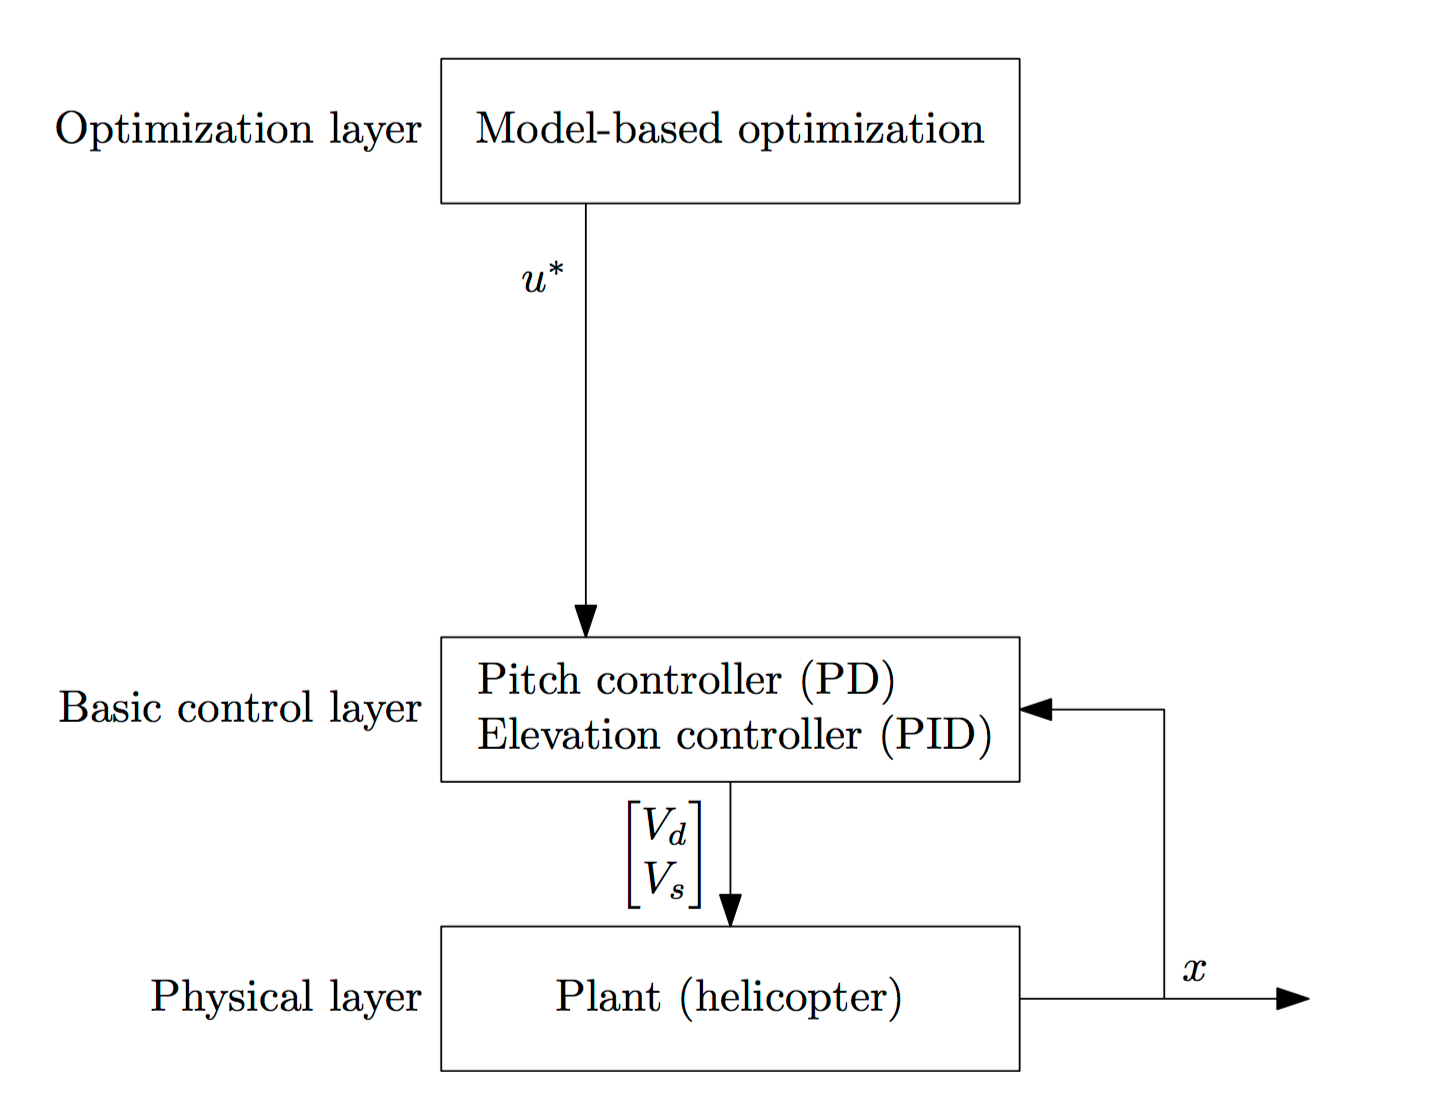
\includegraphics[scale=0.3]{Figur.png}
\caption{Model of the Helicopter with forces and angles}
\label{fig:model2}
\end{center}
\end{figure}


The helicopter can be modeled as three point masses: two representing the two motors at the helicopter head and one mass representing the counterweight as shown in \figref{fig:model}. There are three rotation joints: $p$ denotes the pitch angle of the helicopter head, $e$ denotes the elevation angle and $\lambda$ denotes the travel angle of the helicopter. In \figref{fig:model} all angles are zero. All forces that are not neglected are also showed on \figref{fig:model}. The propeller forces for the front and back propeller are $F_f$ and $F_b$, respectively. They will be given by the following relations:

\begin{subequations}
\label{Fp}
\begin{alignat}{2}
F_f & = K_f V_f\\
F_b & = K_f V_b,
\end{alignat}
\end{subequations}

where $V_f$ and $V_b$ are the voltages supplied to the respective propellers and $K_f$ is the motor force constant. The lift of the helicopter can be determined by the sum of the propeller forces, $F_f + F_b$. The rotation about the pitch axis can be determined by the difference between the propeller forces, $F_f - F_b$. 
\\\\
The gravitational forces from propellers and the counterweight are $F_{g,f}, F_{g,b}$ and $F_{g,c}$, respectively, and given by the following equations
\begin{subequations}
\label{Fg}
\begin{alignat}{2}
F_{g,f} & = F_{g,b} = m_p g \\
F_{g,c} & = m_c g,
\end{alignat}
\end{subequations}
\\
with $m_p$ as the mass of each propeller, $m_c$ as the weight of the counterweight and $g$ is the gravitational constant. 
\\\\
The sum and the difference of the supplied voltages can be defined as
\begin{subequations}
\label{V}
\begin{alignat}{2}
V_s & \equiv V_b + V_f\\
V_d & \equiv V_b - V_f.
\end{alignat}
\end{subequations}
\\
\section{Part II - Optimal Control of Pitch/Travel without Feedback}
In this part we calculate and implement an optimal input sequence that moves the helicopter 180 degrees.

\subsubsection{Problem 1 - Continuous time state}
We write the model on continuous time state space form
\begin{equation}
\mathbf{\dot{x}} = \mathbf{A_c} \mathbf{x} + \mathbf{B_c} \mathbf{u}
\label{linsys}
\end{equation}
where we define the state of the helicopter be described by the vector $\mathbf{x}$: 
\begin{equation}
\mathbf{x} =
\begin{pmatrix}
\lambda \\
r \\
p \\
\dot{p}
\end{pmatrix},
\label{xmat2}
\end{equation}
\begin{equation}
u = p_c
\label{u}
\end{equation}
\\
\subsubsection{Calculation of the relevant matrices}
Equation \eqref{model}, \eqref{system} and \eqref{xmat2} are used to find the matrices $\bold{A_c}$ and $\bold{B_c}$:
\begin{equation}
\bold{A_c} =
\begin{pmatrix}
0 & 1 & 0 & 0  \\
0 & 0 & -K_2 & 0 \\
0 & 0 & 0 & 1 \\
0 & 0 & -K_1K_{pp} & -K_1K_{pd}
\end{pmatrix} 
\label{Amatrix}
\end{equation}
\begin{equation}
\bold{B_c} =
\begin{pmatrix}
0\\
0 \\
0 \\
K_1K_{pp}
\end{pmatrix}.
\label{Bmatrix}
\end{equation}

We are modeling the physical layer of the helicopter. The model includes the state matrix $\bold{A_c}$ \eqref{Amatrix}, the state vector $\bold{x}$ \eqref{xmat2}, the input matrix $\bold{B_c}$ \eqref{Bmatrix}, and the control input u \eqref{u}. This is represented by the physical layer in \figref{fig:model2}. The elevation, e, is not at part of the state vector $\bold{x}$ \eqref{xmat2}. And we will in this task assume e = 0. //

\begin{figure}[h!]
\begin{center}
\centering
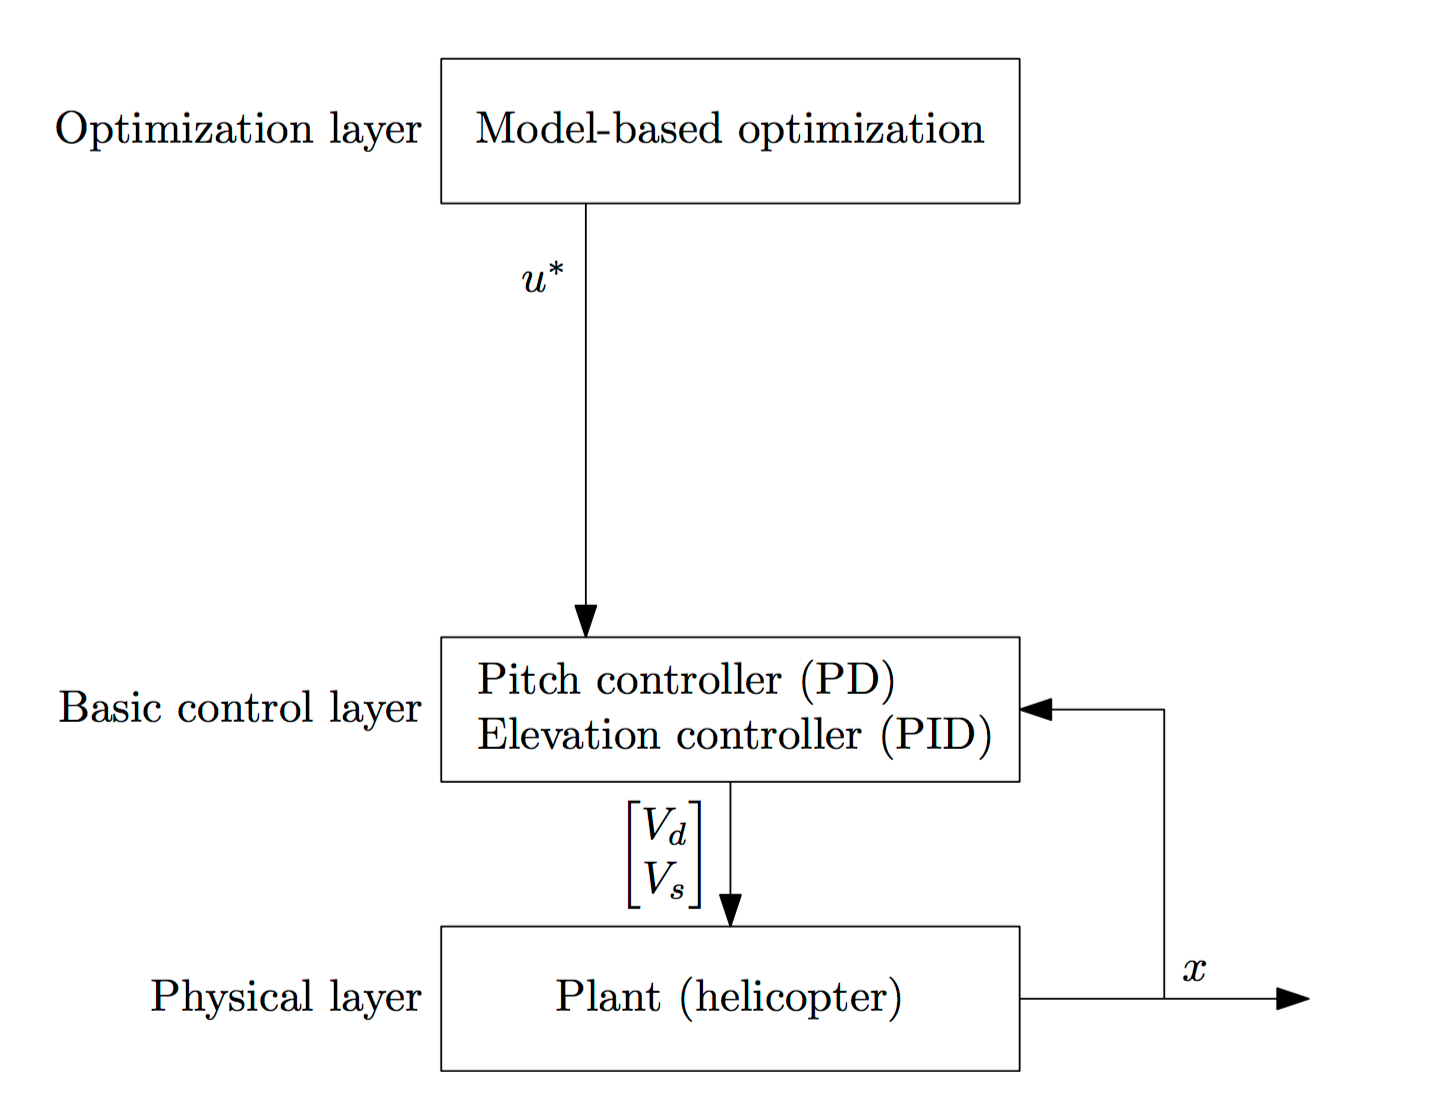
\includegraphics[scale=0.3]{Figur.png}
\caption{Illustration of the layers in the control hierarchy}
\label{fig:model2}
\end{center}
\end{figure}



\subsubsection{Problem 2 - Discretize the model by using the forward Euler method}
The following equations describe the forward Euler method
\begin{subequations}
\begin{alignat}{3}
\dot{x} & = \frac{x_{k+1} - x_k}{\Delta{t}} \\
x_{k+1} & = (\bold{I} + \Delta{t}\bold{A_c})x_k + \Delta{t}\bold{B_c}u_k \\
x_{k+1} & = \bold{Ax_k} + \bold{B}u_k
\end{alignat}
\label{euler}
\end{subequations}
\\
By using \eqref{euler}, we obtain the matrices
\begin{equation}
\bold{A_k} =
\begin{pmatrix}
1 & \Delta{t} & 0 & 0  \\
0 & 1 & -\Delta{t}K_2 & 0 \\
0 & 0 & 1 & \Delta{t} \\
0 & 0 & -\Delta{t}K_1K_{pd} & 1 - \Delta{K_1}K_{pd}
\end{pmatrix}
\quad
\mathrm{and} 
\quad
\bold{B_k} =
\begin{pmatrix}
0\\
0 \\
0 \\
\Delta{t}K_1K_{pp}
\end{pmatrix}.
\label{eulMat}
\end{equation}

\subsubsection{Problem 3 - Calculation of an optimal projectory}






\subsection*{Method}
\subsubsection*{Problem 1}
\subsubsection*{Problem 2}
\subsubsection*{Problem 3}

\subsection*{Results}
\subsubsection*{Problem 1}
\subsubsection*{Problem 2}
\subsubsection*{Problem 3}

\subsection*{Discussion}
\subsubsection*{Problem 1}
\subsubsection*{Problem 2}
\subsubsection*{Problem 3}

\subsection*{Conclusion}

\section{Part III - Optimal Control of Pitch/Travel with Feedback (LQ)}
\subsubsection*{Problem 1}
\subsubsection*{Problem 2}
\subsubsection*{Problem 3}

\subsection*{Method}
\subsubsection*{Problem 1}
\subsubsection*{Problem 2}
\subsubsection*{Problem 3}

\subsection*{Results}
\subsubsection*{Problem 1}
\subsubsection*{Problem 2}
\subsubsection*{Problem 3}

\subsection*{Discussion}
\subsubsection*{Problem 1}
\subsubsection*{Problem 2}
\subsubsection*{Problem 3}

\subsection*{Conclusion}
From this we can conclude that it is not easy to control the helicopter without any form for feedback or a controller. 


\section{Part IV - Optimal Control of Pitch/Travel and Elevation with and without Feedback}

\subsubsection*{Problem 1}
By using \eqref{euler} we get this matrices
\begin{equation}
\bold{A_k} =
\begin{pmatrix}
1 & \Delta{t} & 0 & 0 & 0 & 0 \\
0 & 1 & -\Delta{t}K_2 & 0 & 0 & 0 \\
0 & 0 & 1 & \Delta{t} & 0 & 0 \\
0 & 0 & -\Delta{t}K_1K_{pp} & 1 - \Delta{t}K_1K_{pd} & 0 & 0 \\
0 & 0 & 0 & 0 & 1 & \Delta{t} \\
0 & 0 & 0 & 0 & - K_3K_{ep}\Delta{t} & 1 - K_3K_{ed}\Delta{t}
\end{pmatrix}
\end{equation}
\begin{equation}
\mathrm{and}
\quad
\bold{B_k} =
\begin{pmatrix}
0 & 0 \\
0 & 0 \\
0 & 0 \\
\Delta{t}K_1K_{pp} & 0 \\
0 & 0 \\
0 & K_3K_{ep}\Delta{t}
\end{pmatrix}.
\label{matrices}
\end{equation}




\subsubsection*{Problem 2}
\subsubsection*{Problem 3}
\subsubsection*{Problem 4}
\subsubsection*{Problem 5}
\subsubsection*{Problem 6}

In this exercise we tested for several different constraints for the travel rate and the elevation rate. 

\subsection*{Method}
\label{S:3}
\subsubsection*{Problem 1}
\subsubsection*{Problem 2}
\subsubsection*{Problem 3}
\subsubsection*{Problem 4}
\subsubsection*{Problem 5}
\subsubsection*{Problem 6}

\subsection*{Results}
\label{S:4}

\subsubsection*{Problem 1}
\subsubsection*{Problem 2}
\subsubsection*{Problem 3}
\subsubsection*{Problem 4}
\subsubsection*{Problem 5}
\subsubsection*{Problem 6}

\subsection*{Discussion}
\label{S:5}

\subsubsection*{Problem 1}
\subsubsection*{Problem 2}
\subsubsection*{Problem 3}
\subsubsection*{Problem 4}
\subsubsection*{Problem 5}
\subsubsection*{Problem 6}

\subsection*{Conclusion}
\label{S:6}

\section{Conclusion}

\newpage

\section{MATLAB Code}\label{sec:matlab}
This section should contain your MATLAB code. DO NOT attach files posted online (that you didn't write). Note that the method used to input code below does not look as pretty when the lines are too long.

%\subsection{plot\_constraint.m}\label{sec:plot_constraint_m}
%\lstinputlisting{code/plot_constraint.m}
%% References
%%
%% Following citation commands can be used in the body text:
%% Usage of \cite is as follows:
%%   \cite{key}          ==>>  [#]
%%   \cite[chap. 2]{key} ==>>  [#, chap. 2]
%%   \citet{key}         ==>>  Author [#]

%% References with bibTeX database:

\bibliographystyle{model1-num-names}
\bibliography{sample.bib}

%% Authors are advised to submit their bibtex database files. They are
%% requested to list a bibtex style file in the manuscript if they do
%% not want to use model1-num-names.bst.

%% References without bibTeX database:

% \begin{thebibliography}{00}

%% \bibitem must have the following form:
%%   \bibitem{key}...
%%

% \bibitem{}

% \end{thebibliography}


\end{document}